\section{Methodology and Implementation}
	
	\subsection{Hardware ${}^{\ref{HardwareSource}}$ }

	\begin{enumerate}[topsep=-2pt, itemsep=2pt]
		\item \textbf{Raspberry Pi 3 Model B:} The Raspberry Pi 3 is a hobbyist microcontroller board which can be used for a variety of embedded systems projects. 
		
			It's specifications ${}^{\cite{RPi3BSpecs}}$ include:
			\begin{description}[font=\quad $\circ$, topsep=-2pt, itemsep=2pt]
				\item Broadcom BCM2837 64bit ARMv7 Quad Core Processor powered Single Board computer running at 1.2GHz
				\item 1 GB RAM
				\item BCM43143 WiFi on board
				\item 4 USB 2.0 ports
				\item 40 GPIO pins${}^{\ref{fig: Raspberry Pi 3B pin diagram}}$ (General Purpose Input Output)
				\item Full HDMI port
				\item Micro SD card slot (an 8Gb SanDisk MicroSD was used)
			\end{description}
			
			\begin{figure}[!h]
				\centering
				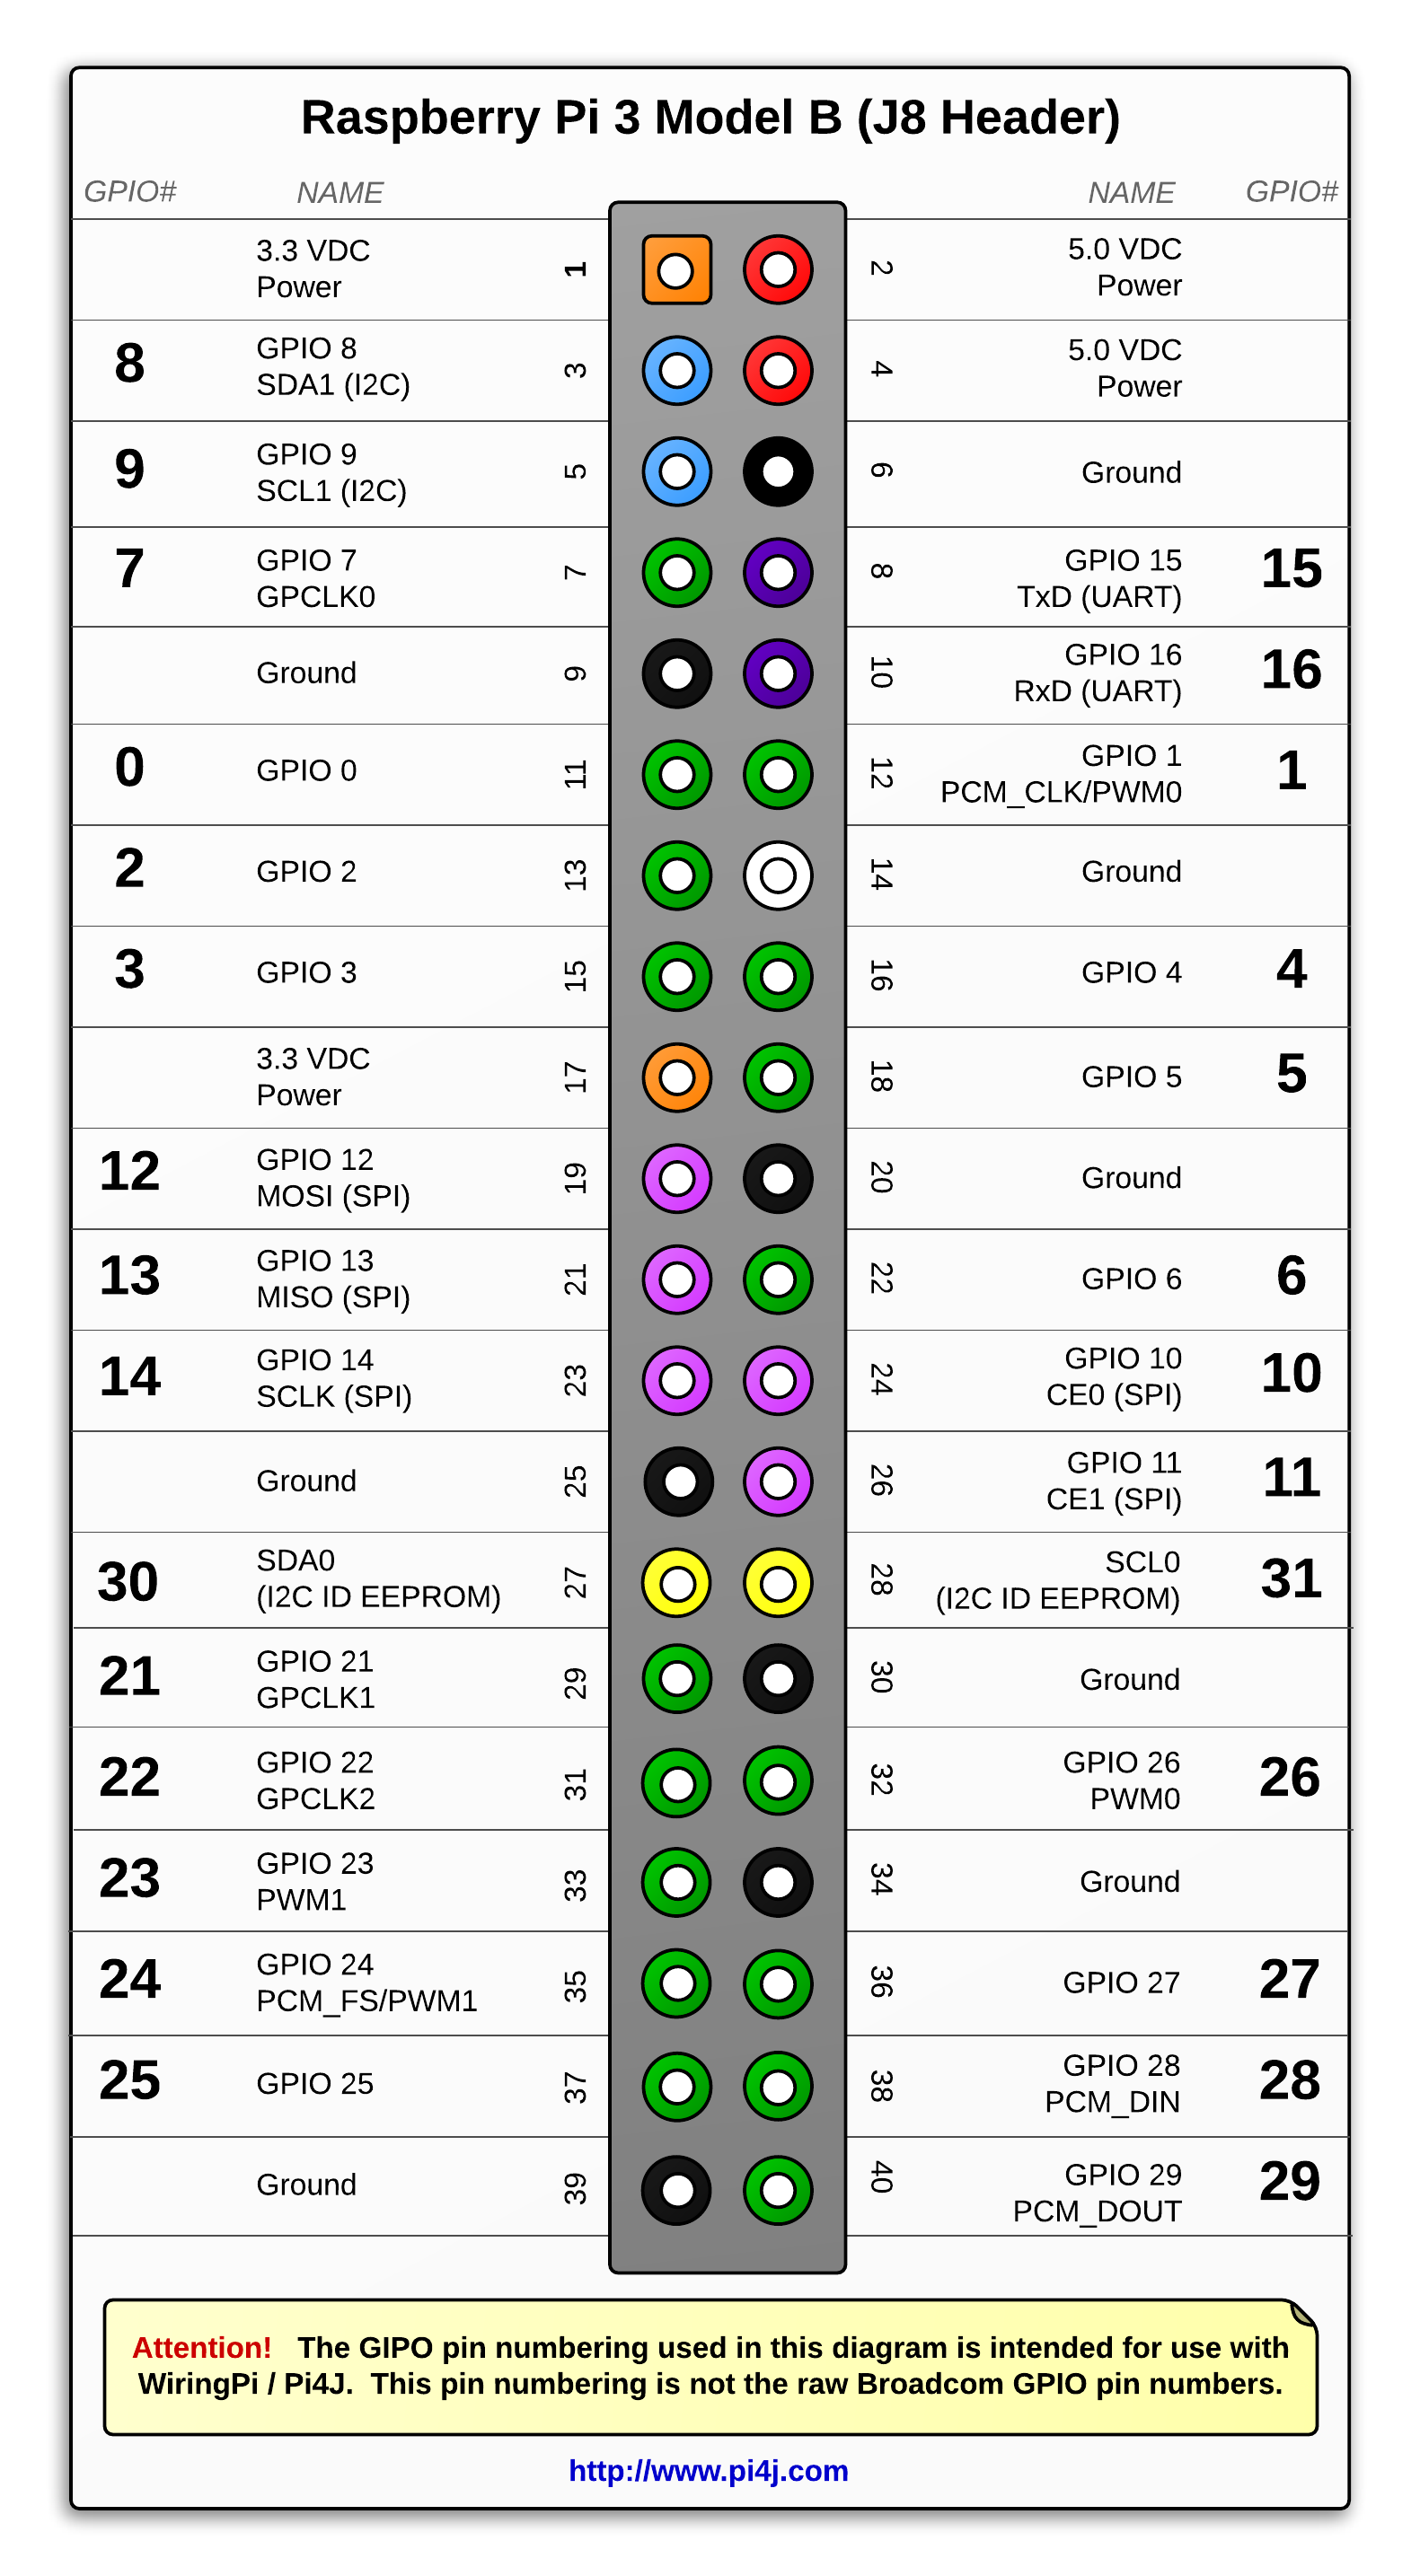
\includegraphics[width=0.42\linewidth]{"./raspberry-pi-3b-pin-diagram-j8header.png"}
				\caption{Raspberry Pi 3B pin diagram}
				\label{fig: Raspberry Pi 3B pin diagram}
			\end{figure}
			
			
			\footnotetext[1]{\label{HardwareSource} Most hardware for this project was obtained from specialty electronic stores around Mumbai. The Raspberry Pi 3B was borrowed from Prof. Bhole, Computers and Information Techonolgy Department, VJTI. We did our best not to alter his existing configurations.}
		
		
		
			
		\clearpage
		
		\item \textbf{Wheels and motors:} the robot moves using two wheels each driven by a 300 RPM DC motor. These DC motors are connected with L293D IC which provides and H bridge to turn one motor and other off or both simultaneously in same direction or different direction. 
		
		
		\item \textbf{L293D Motor Driver:} a quadruple high-current half-H driver. The L293D is designed to provide bidirectional drive currents of up to 600-mA at voltages from 4.5 V to 36 V. This allows the wheels to move in both directions and also turn left and right. ${}^{\cite{L293D_MotorDriver}}$
		
		
			We connect this driver${}^{\ref{fig: L293D Motor Driver pin diagram}}$ to the following pins of the Raspberry Pi:
	
			\tabulinesep=6pt	% Source: tex.stackexchange.com/a/207146/110560
			\begin{longtabu} to \textwidth {| c | c | } \hline
				\centering 
				Raspberry Pi 3B & L293D \\ \hline
				GPIO 29 (pin 40) & VCC \\ 
				GPIO 28 (pin 38) & GND \\ 
				GPIO 26 (pin 32) & GND \\ 
				Ground (pin 30) & GND \\ \hline
				\caption{Connections of Raspberry Pi to L293D Motor Driver}
			\end{longtabu}
			
			\begin{figure}[!h]
				\centering
				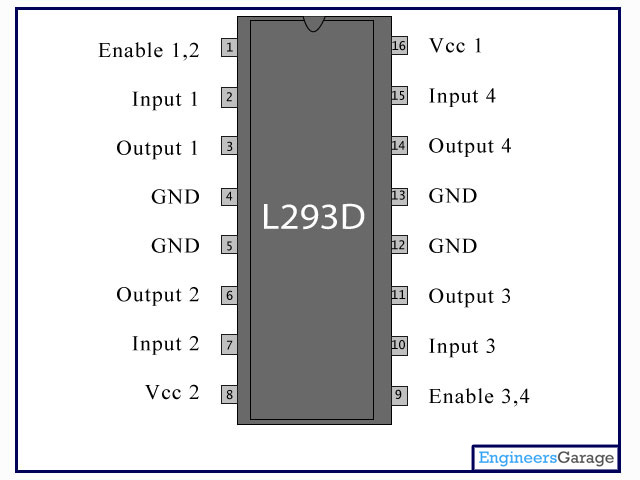
\includegraphics[width=0.5\linewidth]{"./L293D.jpg"}
				\caption{L293D Motor Driver pin diagram}
				\label{fig: L293D Motor Driver pin diagram}
			\end{figure}
			
			
			 \begin{figure}
				\centering
				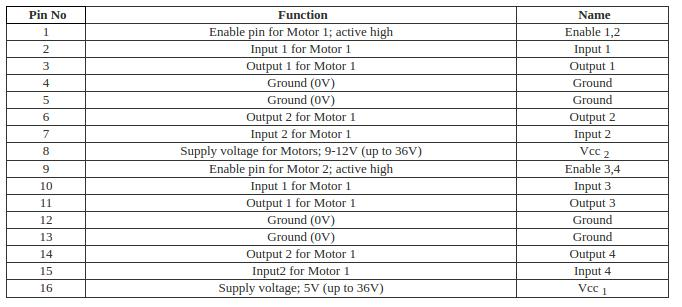
\includegraphics[width=\linewidth]{L293D_pin_description}
				\caption{L293D pin description}
				\label{fig:L293D_pin_description}
			\end{figure}

			 
		 
		\item \textbf{IR sensors:} In the rover, IR sensors are used to perform line-following on black or white striped lines. 
		
			IR sensors work on the principle of reflectance where there is one transmitter and one receiver. The transmitter transmits InfraRed rays which are received by the receiver to complete the circuit, due to which current flows through it. ${}^{\ref{fig:IR_transmitter_reciever}}$
			
			\begin{figure}
				\centering
				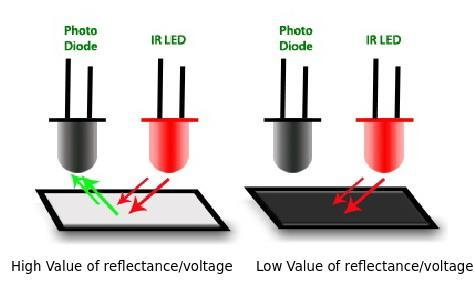
\includegraphics[width=0.5\linewidth]{IR_transmitter_reciever}
				\caption{The working of IR sensors}
				\label{fig:IR_transmitter_reciever}
			\end{figure}
			
			Dark colors are good absorber of rays, and they reflect very few of the IR rays falling on it. ${}^{\ref{fig:IR_transmitter_reciever2}}$ Due to this phenomenon, using a dark color as the background and white color as line allows to distinguish the path from the background as only white color will be detected by the sensors. 
			
			\begin{figure}
				\centering
				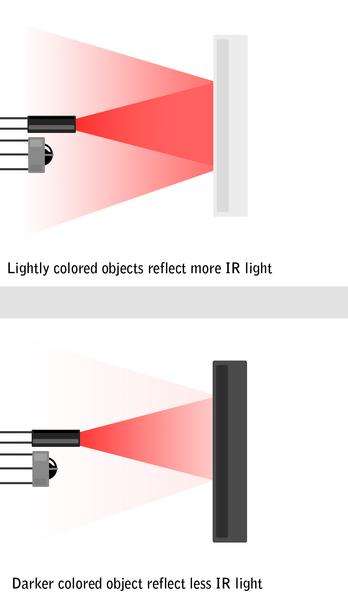
\includegraphics[width=0.4\linewidth]{IR_transmitter_reciever2}
				\caption{Dark colors absorb more light}
				\label{fig:IR_transmitter_reciever2}
			\end{figure}



	\end{enumerate}
	
	